\section{Results}
\label{sec:results}

\paragraph{Leakage exists on a task-capable backbone.} On the DGCNN backbone (BNCI2014\_001 fold-0), the
graph and node objects carry strong, significant, and spatially stable leakage: the graph proxy is
$\approx 8\times$ and the node proxy $\approx 15\times$ the permutation mean, clearing the null in $3/3$
seeds, with a node-leakage map highly reproducible across seeds (mean pairwise correlation $\approx 0.945$).
This is the first such audit on a backbone that \emph{also} learns the task (Table~\ref{tab:leakage_audit}).

% Table 2 — DGCNN leakage audit (CIGL_25, BNCI2014_001 fold-0). Draft; values from RESULTS_TABLES_DRAFT.md (T2).
\begin{table}[t]
\centering
\caption{Source-only leakage audit on the DGCNN backbone (BNCI2014\_001 fold-0). The proxy is compared to a
retrained within-label permutation null; \texttt{clears} = significant in 3/3 seeds. Edge is skipped
(static adjacency, \texttt{edge\_logits=None}).}
\label{tab:leakage_audit}
\small
\begin{tabular}{lcccc}
\toprule
Object & kl\_mean & perm\_mean & $p$ & clears (seeds) \\
\midrule
graph $Z_g$ & $\approx 1.26$ ($\approx 8\times$ perm)  & $\approx 0.16$  & 0.020 & 3/3 \\
node $Z_v$  & $\approx 0.52$ ($\approx 15\times$ perm) & $\approx 0.034$ & 0.020 & 3/3 \\
\bottomrule
\end{tabular}

\vspace{2pt}
\footnotesize Node-leakage map stable across seeds (mean pairwise corr.\ $\approx 0.945 \gg$ null q95 $\approx 0.20$).
\end{table}


\paragraph{Fixed regularizer reduces leakage at task retention --- two datasets.} On \textbf{BNCI2014\_001}
(primary folds 1--8; fold-0 is the development fold and is excluded), the fixed \texttt{graph\_node\_010}
passes all four source-only criteria in every primary fold while meeting the source-task retention gate
(absolute drop $\le 0.02$); graph and node proxy reductions and their fold-level bootstrap confidence
intervals are in Table~\ref{tab:bnci2014}. On \textbf{BNCI2015\_001} (all 12 LOSO folds), the same fixed candidate is
ERM-adequate, leakage-bearing, and leakage-reducing in $12/12$ folds, meets the retention gate in $11/12$
folds (one fold misses the per-fold threshold; the dataset-level gate passes), and holds the
evaluation-only target guardrail in $12/12$ folds, yielding
$\texttt{confirmed\_with\_target\_guardrail} = \texttt{true}$; reductions and CIs are in
Table~\ref{tab:bnci2015}. Figure~\ref{fig:retention} plots every fold's reduction against its source-task
retention.

% Table 3 — BNCI2014_001 confirmation (CIGL_29; primary folds 1-8; fold-0 = dev, excluded).
% Draft; means/ranges from RESULTS_TABLES_DRAFT.md (T3); 95% CIs from STATISTICAL_SUMMARY_DRAFT.md
% (fold-level bootstrap, seed 0, 10000 resamples, percentile).
\begin{table}[t]
\centering
\caption{BNCI2014\_001 confirmation of the fixed \texttt{graph\_node\_010} (primary folds 1--8; fold-0 is
the development fold, excluded). bAcc = balanced accuracy (chance 0.25); KL reduction = $(\mathrm{ERM}-
\mathrm{reg})/\mathrm{ERM}$ of the posterior-KL proxy. 95\% CIs are fold-level bootstrap. ``retain'' = source
drop $\le 0.02$. Edge skipped.}
\label{tab:bnci2014}
\small
\begin{tabular}{lc}
\toprule
Quantity & Value \\
\midrule
fold group / $n_{\mathrm{folds}}$        & primary folds 1--8 / 8 \\
ERM source bAcc (mean [range])           & 0.484 [0.457, 0.508] \\
reg source bAcc (mean, 95\% CI)          & 0.488 [0.471, 0.505] \\
source retention (drop $\le 0.02$)       & 8/8 \\
graph KL reduction (mean, 95\% CI; range)& 44.0\% [39.5, 49.0]; 35--58\% \\
node KL reduction (mean, 95\% CI; range) & 36.9\% [33.6, 40.3]; 31--45\% \\
ERM leakage clears null / reg reduces $\ge$30\% & 8/8 / 8/8 \\
target guardrail (drop $\le 0.05$)       & 8/8 \\
reg leakage still clears null            & every fold (partial, not elimination) \\
edge status / decision                   & skipped / \textbf{A} \\
\bottomrule
\end{tabular}
\end{table}

% Table 4 — BNCI2015_001 confirmation (CIGL_31; all 12 LOSO folds).
% Draft; means/ranges from RESULTS_TABLES_DRAFT.md (T4); 95% CIs from STATISTICAL_SUMMARY_DRAFT.md
% (fold-level bootstrap, seed 0, 10000 resamples, percentile).
\begin{table}[t]
\centering
\caption{BNCI2015\_001 confirmation of the same fixed \texttt{graph\_node\_010} (all 12 LOSO folds). bAcc
chance 0.50. 95\% CIs are fold-level bootstrap. One fold (fold9, $+0.024$) misses the per-fold retention
threshold while the dataset-level gate passes. Edge skipped.}
\label{tab:bnci2015}
\small
\begin{tabular}{lc}
\toprule
Quantity & Value \\
\midrule
fold group / $n_{\mathrm{folds}}$        & all LOSO folds / 12 \\
ERM source bAcc (mean [range])           & 0.706 [0.682, 0.734] \\
reg source bAcc (mean, 95\% CI)          & 0.700 [0.693, 0.707] \\
source retention (drop $\le 0.02$)       & 11/12 (fold9 $+0.024$) \\
graph KL reduction (mean, 95\% CI; range)& 66.2\% [60.6, 71.0]; 43--77\% \\
node KL reduction (mean, 95\% CI; range) & 51.9\% [47.8, 55.6]; 37--61\% \\
ERM adequacy / leakage / reg reduces $\ge$30\% & 12/12 / 12/12 / 12/12 \\
target guardrail (drop $\le 0.05$)       & 12/12 \\
reg leakage still clears null            & every fold (partial, not elimination) \\
edge status / decision                   & skipped / \textbf{A} (\texttt{confirmed\_with\_target\_guardrail=true}) \\
\bottomrule
\end{tabular}
\end{table}


\begin{figure}[t]
  \centering
  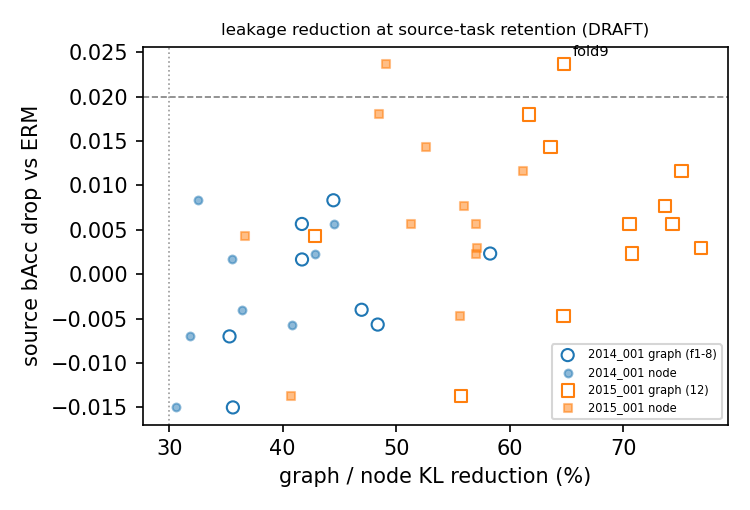
\includegraphics[width=0.62\linewidth]{figures/fig2_reduction_vs_retention_draft.png}
  \caption{\textbf{[DRAFT, from data]} Per-fold graph/node KL reduction (\%) vs source bAcc drop relative to
  ERM, for BNCI2014\_001 (folds 1--8) and BNCI2015\_001 (12 folds). The $y$-axis is a \emph{retention} axis:
  near-zero drop means the task is retained, not improved. The dashed line is the retention gate
  ($\text{drop}\le 0.02$); the single BNCI2015\_001 point above it (fold9, $+0.024$) is annotated. Values
  from the per-fold confirmation logs.}
  \label{fig:retention}
\end{figure}

\paragraph{Partial, not total.} In every confirmation fold the \emph{regularized} leakage still clears the
null --- CIGL reduces the proxy substantially (see Tables~\ref{tab:bnci2014}--\ref{tab:bnci2015}) but does
not eliminate the leakage. We report reduction, not removal.
